

\documentclass{article}
\usepackage{graphicx}


\title{Status Of Old Computer Vision Code}
\date{11/3/15}
\author{Jon Dixon, Julian Brackins}

\begin{document}
	\maketitle
	\newpage
	
	\section{Introduction}
	The purpose of this report is to give a brief overview of the current status of the existing code from the 2014-2015 landing pad team's repository. Fortunately, it appears that much of the code is reusable. If not in full, parts of the code can be pulled from the repository to get the ball rolling. In the report, we'll go through where to find the existing code in the repository, and what it's currently capable of.
	
	\section{Location in Repository and Building Source}
	The code being discussed throughout is in the GitHub repository under the directory landingpad/2014-2015/led/. To run this code on your local machine (assuming you have opencv installed as well as the latest compilers) navigate to the above directory, and type 'cmake .'. Then, run make. Once you've done this, you can run the code with './tracker'. Assuming you're on your school laptop, it'll automatically access the front-facing camera, and you'll see a happy little picture of your smiling face! I'm assuming that you're happy, since you've just succeeded in getting the software to run. As this runs, you may notice that it draws some circles and coordinates on the video feed. This overlay is meant to point out the positions of the RGB blobs in the frame. We've taken the large printout of the AR tag and RGB blobs that the team used last semester, and tested the code with it. Fortunately, it works! You can see the results of this in the image below.
	
	\begin{figure}[p]
		\centering
		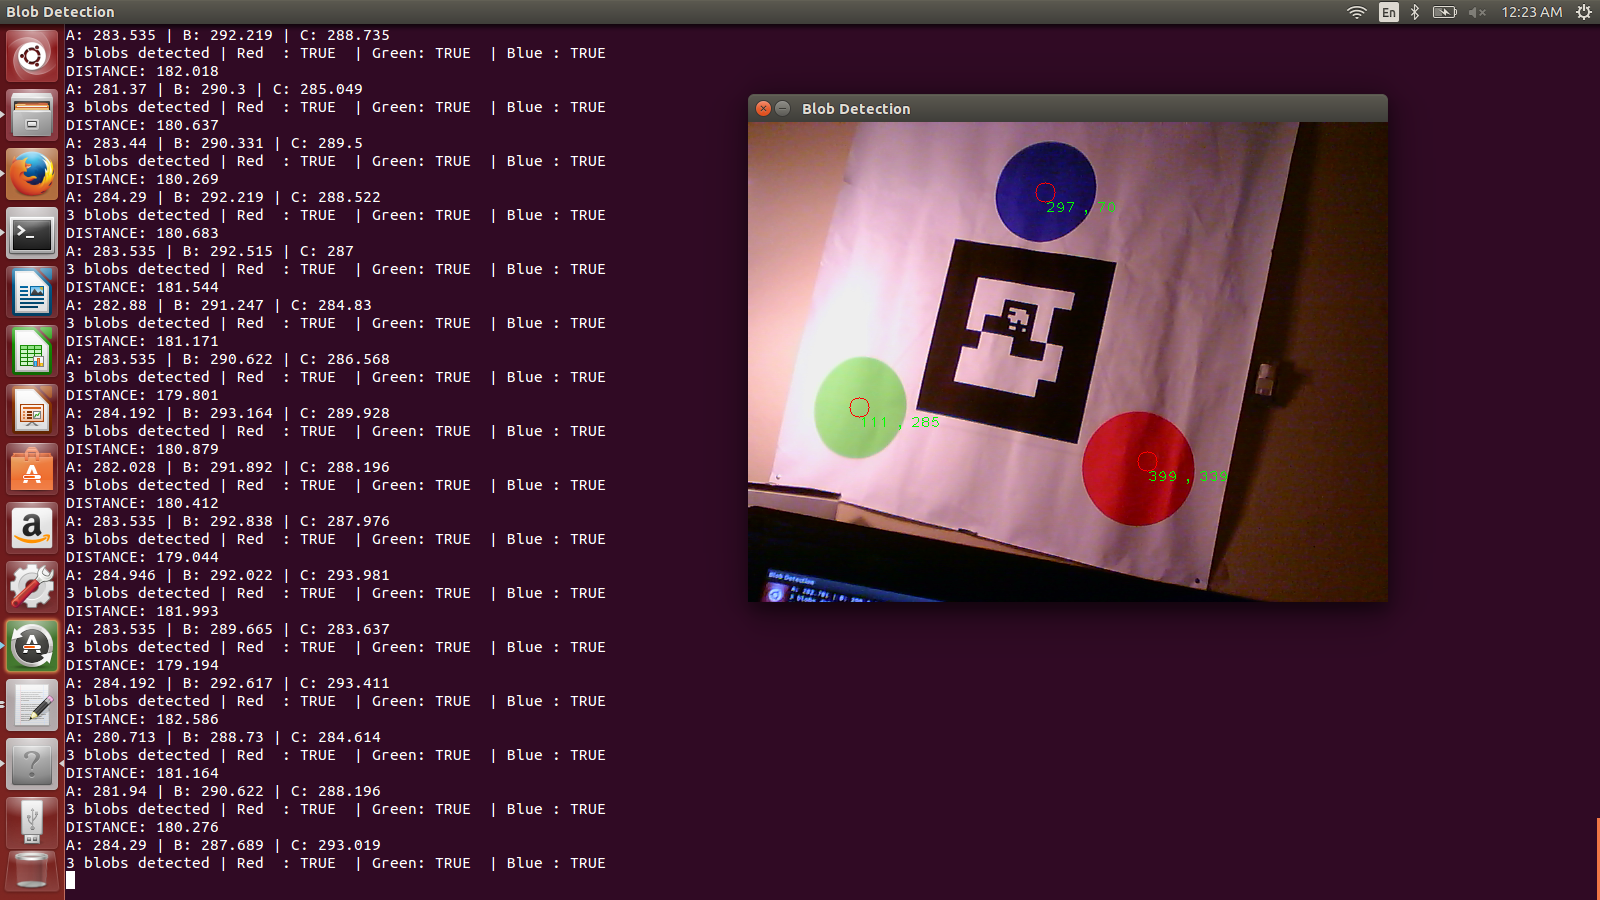
\includegraphics[width=0.8\textwidth]{coolpic.png}
		\caption{Blobs Detected}
	\end{figure}
	
	\section{Next Steps}
	Since the existing code outputs a correct distance in centimeters, the next step will to be able to detect the angle of the image. This will allow us to determine orientation. Since we have working code, we should just be able to clean it up, and copy it over into a new branch of our current repository. From there, we will begin to develop orientation detection!
	
\end{document}